%% \section{Delta Dictionaries}
\section{Implementation}
\label{sec:DD}

\newcommand{\ddExampleScale}
  %% {0.45}
  {0.50}
  %% {0.55}

\begin{figure}

\centering

%% \begin{figure}[b] %% [H]
\begin{subfigure}[h]{\columnwidth}
  \centering
  \begin{tikzpicture}[nodes = {align = left}]
    \node [scale=\ddExampleScale]
    {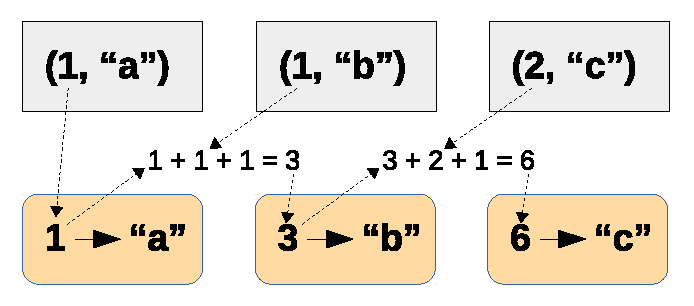
\includegraphics{figs/mech-2-very-short.eps}};
  \end{tikzpicture}
  \caption{An example delta dictionary.}
  %% \caption{What mapping is represented by the \dd~ $\dictP$?}
  \label{fig:dd-example}
\end{subfigure}
%% \end{figure}

\vspace{0.15in}

\begin{figure}[b] %% [H]
  \centering
  \begin{tikzpicture}[nodes = {align = left}]
    \node [scale=.4]
    {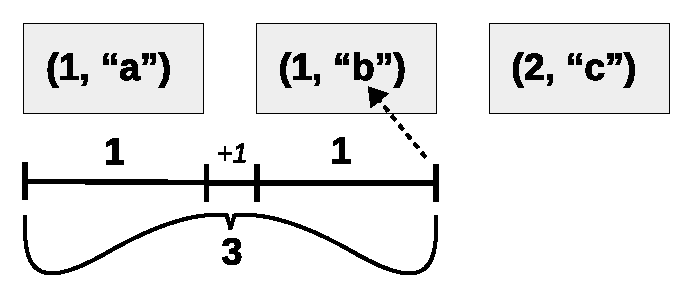
\includegraphics{figs/find-3-very-short.eps}};
  \end{tikzpicture}
  \caption{How do we find key $3$?} %% in the \dd?}
  \label{fig:dd-example-find}
\end{figure}

\vspace{0.15in}

\begin{figure}[H]
  \centering
  \begin{tikzpicture}[nodes = {align = left}]
    \node [scale=.4]
    {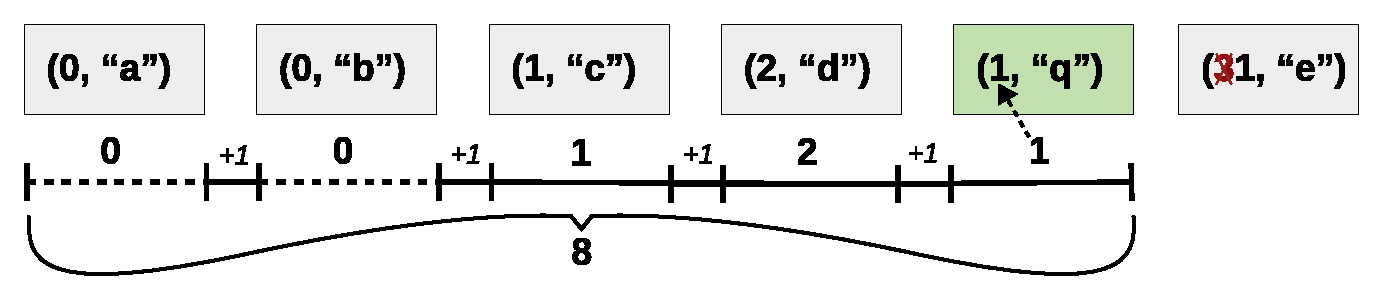
\includegraphics{figs/insert-8.eps}};
  \end{tikzpicture}
  \caption{How do we insert a mapping from key $8$ to value "q"?}
  \label{fig:find-6}
\end{figure}


\caption{Example delta dictionary operations.}
\end{figure}


Our implementation of delta dictionaries and corresponding proofs are formalized in Agda and available in the anonymous supplementary materials.

%% \subsection{Delta Indexing}
%% \subsection{Key Types and Deltas}
\subsection{Deltas and Key Types}

Borrowing from association lists, \dds{} use a list-of-pairs, where the first item in each list represents a key and the second is the literal value that is mapped to the represented key.
%
Unlike association lists, the natural number that represents the key is not its literal value.

In order to allow multiple key types, while relying on useful properties of natural numbers under the hood, \dds{} accept a typeclass argument representing a bijection
%
between the key type and the naturals, and use this bijection to convert keys to and from naturals. This is discussed further in \emph{\textbf{Bijections to Natural Numbers}}.

In order to maintain canonical order, while ensuring that every natural number is valid as the first item in a pair, that number must represent the non-negative difference between the key it represents and the previous key.
%
We call this number a \emph{delta}. % , alluding to the \emph{delta encoding} technique more commonly harnessed for performance optimization.
%
As described so far, a $0$ offset would correspond to a duplicate key.
%
To prevent duplicate keys from being represented, a delta is actually the offset minus $1$: a delta of $0$ indicates an offset (from the previous key) of $1$, a delta of $2$ indicates an offset of $3$, and so on.
%
The head of the list, however, does not follow the ``minus $1$'' rule: so the first ``delta'' is interpreted literally, \ie{}~it represents the key value exactly.

\autoref{fig:dd-example} depicts the \dd{} corresponding to the example from \autoref{sec:Introduction}.

%% \subsection{Bijections to the naturals}
%% \label{sec:DD:bij}
\parahead{Bijections to Natural Numbers}

In our implementation, each key is represented by a natural number, so that we can use addition, subtraction, and successor operations in order to define deltas.
%
There may be an algebraic structure more general than the natural numbers which satisfies these requirements, but for practical purposes, working with naturals
%
is easier for both the implementer and the client. In Agda, the bijection typeclass accepts a \texttt{convert} function, as well as proofs that \texttt{convert}
%
is injective and surjective, and the inverse function is defined by the library using the proof of surjectivity.\footnote{\hspace{0.01in}%
%
Without surjectivity, a binding for an unmapped natural either invalidates the \dd---violating \Total---or is ignored, in which case its presence or absence does not affect the semantic meaning---violating \Extensional.
%
}
%
We demonstrate this in Agda by
%
providing an instance of the bijection typeclass for integers ($25$ lines of code).

Most types that are suitable for use as keys in the first place, especially strings and countable numeric types, can be bijected to the naturals,
%
though doing so may be onerous. Finite types, such as characters, are suitable as keys, but cannot be bijected to the naturals---%
%
simultaneously achieving \Total{} and \Extensional{} for a dictionary over finite types may require a custom-made dictionary data type.

\Ddls{} are canonically ordered, but by the natural ordering of the naturals, which, depending on the choice of bijection, may correspond to an unnatural
%
ordering of the key type. As such, we do not expose the ordering to the client---functions such as \texttt{destruct} and \texttt{toList} produce results
%
that are in arbitrary order from the client's perspective.

%%, and so from the client's perspective, the \dd{} is unordered.

\subsection{Lookup, Insertion, and Destruction}
\label{sec:DD:basics}

\newcommand{\twoChars}
  {\hspace{0.145in}}
\newcommand{\fourChars}{\twoChars\twoChars}
\begin{figure}
%% \begin{figure*}
%% TODO using alltt temporarily, to inline Delta.agda directly
%% \input{code/lkupins.hs}
\begin{alltt}
\input{code/Delta.agda}
\end{alltt}
\caption{Delta dictionary operations.}
\label{fig:agda}
%% \end{figure*}
\end{figure}


\autoref{fig:dd-example-find} and \autoref{fig:dd-example-insert} illustrate example lookup and insert operations.
%
These proceed largely as they would for association lists, but working indirectly with keys encoded as natural numbers and, furthermore, differences between these numbers.

\autoref{fig:agda} presents concrete implementations for lookup (\ie{} \texttt{\_\altLAng\_\altRAng}), insert (\ie{} \texttt{\_,,\_}), and \texttt{destruct} in Agda.
%
Notice that we choose to parameterize the \texttt{Delta} module by key type \verb+K+ and bijection \verb+bij+ to the naturals; the operations are parameterized by value-binding type \verb+V+.
%
%Having to treat the first delta differently than the rest (literally rather than relatively) is the source of the somewhat technical---through simple---details.

The helper function \verb+delta+ computes the delta, \ie{} the offset minus $1$, between two distinct numbers.
%
Given that, lookup is straightforward. The insert function is also fairly straightforward.
%
If the delta to insert is less than the delta of the first pair, then we place the delta to insert as the first pair of the new list, and
%
the original first pair will be the second pair of the new list, but using the delta between its original value and the inserted delta.
%
If the first pair is an exact match, then we simply replace the old value with the new one.
%
\verb+destruct+ simply pops the head off the list, and then augments the next key by the offset.

%% \cite[Facts about weak maps]{FMapFacts}
%
The Coq Standard \citet[Facts about weak maps]{FMapFacts} describes key metatheory about dictionaries, including that for lookup, insert, and \verb+destruct+.
%
Our Agda mechanization proves the relevant subset of this metatheory. Some of the metatheory in the Coq treatment involves concepts not relevant to our treatment,
%
especially multiple distinct notions of equality. Also, since we do not expose mapping order to the client via our interface,
%
we do not prove any of the theorems pertaining to ordering (\ie{} those that are not ``weak'').


\subsection{Additional Operations}

Our Agda mechanization also defines key deletion, union, map, and to/from-list operations, along
with appropriate metatheory (not reproduced here).



%% \subsection{Core properties}
%% \section{Properties}
\subsection{Properties}
\label{sec:DD:props}

We now consider properties about delta dictionaries, starting with the four design goals identified in \autoref{sec:Introduction}.
%
Theorems below are proven in Agda.
%
Recall that key type \verb+K+ is a module parameter and is implicitly bound in the type \verb+DD V+.

% The \SemInj~ and \EqDec~ theorems, a destruction theorem, and analogs to the \emph{structural properties} \emph{contraction} and \emph{exchange} are defined below, and proven in Agda.

%% \subsection{Design Goals}
%% \parahead{Design Goals}

\begin{remark}[\SemTot]
%
\textnormal{This property cannot be formally defined---rather its truth is apparent from the fact that the other theorems do not require their \dd~ arguments to be refined with validity premises.}
%
\end{remark}

\begin{theorem}[\SemInj]
\label{thm:SemInj}
\justIndent
\begin{alltt}
  \altFAll\{V\} \{dd1 dd2 : DD V\} \altRArr
    ((k : K) \altRArr dd1 \altLAng k \altRAng == dd2 \altLAng k \altRAng) \altRArr
    dd1 == dd2
\end{alltt}
\end{theorem}

\begin{theorem}[\EqDec]
\label{thm:EqDec}
\justIndent
\begin{alltt}
  \altFAll\{V\} (dd1 dd2 : DD V) \altRArr
    ((v1 v2 : V) \altRArr v1 == v2 \altOr v1 \altNE v2) \altRArr
    dd1 == dd2 \altOr dd1 \altNE dd2
\end{alltt}
\end{theorem}

%% \begin{theorem}[\EzDstr]
\begin{theorem}[Not-So-Easy Destructibility]
\label{thm:EzDstr}
\justIndent
\begin{alltt}
  \altFAll\{V\} \{dd dd' : DD V\} \{k : K\} \{v : V\} \altRArr
    (destruct dd == None \altRArr dd == \altEmpty)
      \altAnd
    (destruct dd == Some ((k , v) , dd') \altRArr
      (k \altNIn dd' \altAnd dd == dd' ,, (k , v))
\end{alltt}
\end{theorem}

%% \subsection{Contraction and Exchange}
%% \parahead{Contraction and Exchange for Dictionaries}

%\rkc{Two common properties for PL metatheory.}

\noindent
%
We discuss why destruction is ``not-so-easy'' in detail below.

Lastly, we prove analogs to the \emph{structural properties} \emph{contraction} and \emph{exchange}.

% The \SemInj~ and \EqDec~ theorems, a destruction theorem, and analogs to the \emph{structural properties} \emph{contraction} and \emph{exchange} are defined below, and proven in Agda.

\begin{theorem}[Dictionary Contraction]
\label{thm:cont-dicts}
\justIndent
\begin{alltt}
  \altFAll\{V\} \{dd : DD V\} \{k : K\} \{v v' : V\} \altRArr
    dd ,, (k , v') ,, (k , v) == dd ,, (k , v)
\end{alltt}
\end{theorem}

\begin{theorem}[Dictionary Exchange]
\label{thm:exch-dicts}
\justIndent
\begin{alltt}
  \altFAll\{V\} \{dd : DD V\} \{k1 k2 : K\} \{v1 v2 : V\} \altRArr
    k1 \altNE k2 \altRArr
    dd ,, (k1 , v1) ,, (k2 , v2) ==
    dd ,, (k2 , v2) ,, (k1 , v1)
\end{alltt}
\end{theorem}

\parahead{The Difficulty of Destruction}

\SemInj{} requires canonical ordering and deduplication, and \SemTot{} means that the canonical order and deduplication have to come from
how the data is interpreted rather than how it is organized. The non-literal way in which key data is interpreted means that it is not
safe for client code to work with the raw data directly---rather, all interaction with the data must be
encapsulated in library functions.

Unfortunately, this includes \emph{destruction}; an interaction which
normally goes through the very natural, elegant, and well-supported mechanism of pattern matching is now
only available through the library function \verb+destruct+. \autoref{thm:EzDstr} proves that this function
destructs the \dd{} in essentially the same way that a case expression destructs a list of pairs (although
the order in which bindings are plucked away is arbitrary from the client's perspective).

\verb+destruct+ achieves the same purpose as typical pattern matching (albeit more awkwardly), but because it
does not harness the primitive notions of pattern matching and structure, it does not establish structural
decrease on the dictionary object, which may break out-of-the-box structural recursion in the likely case
of recursion on \verb+dd'+. To enable manual establishment of structural recursion, via an extra parameter that
explicitly tracks the dictionary length, we provide another theorem:

\begin{alltt}
  extend-size :
    \altFAll\{V\} \{dd : DD V\} \{k : K\} \{v : V\} \altRArr
      k \altNIn dd \altRArr
      || dd ,, (k , v) || = 1 + || dd ||
\end{alltt}

Although possible, manually establishing termination is painful, especially given that it is not necessary
for {\sal}s or {\cal}s. Thus \dds~ fail at \EzDstr, although they are still better than {\fpf}s in this
regard, seeing as it is not only hard but impossible to destruct {\fpf}s.

Is it possible to have a data structure that possesses all four properties?
Not likely. As mentioned above, the combination of \SemInj{} and \SemTot{} essentially
necessitates that the data in the data structure be interpreted in a non-literal way, which in turn
makes it dangerous for client code to mess with the raw data. As such, we believe we have uncovered an
inherent trade-off between desirable properties. In cases where \SemTot{} and \EqDec{} are critical,
and there is little to no need to destruct dictionaries, \dds{} seem to be a clear winner over
the conventional solutions. But in cases where \SemTot{} is not so important,
but inspection or destruction are, {\cal}s may be a preferable.
